
\begin{figure*}[t!]
\centering
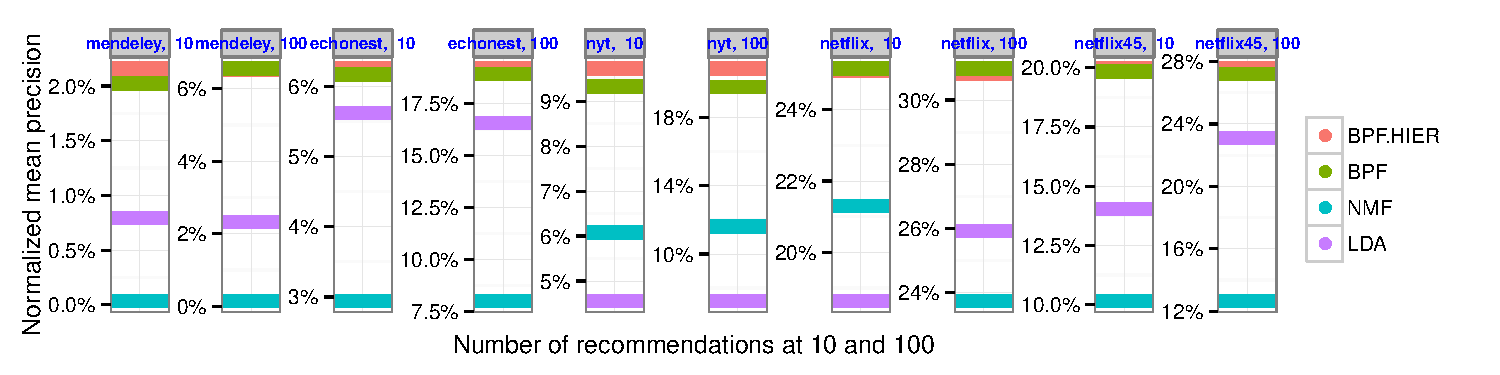
\includegraphics[width=\textwidth]{./figures/meanprecision2.pdf}\\               
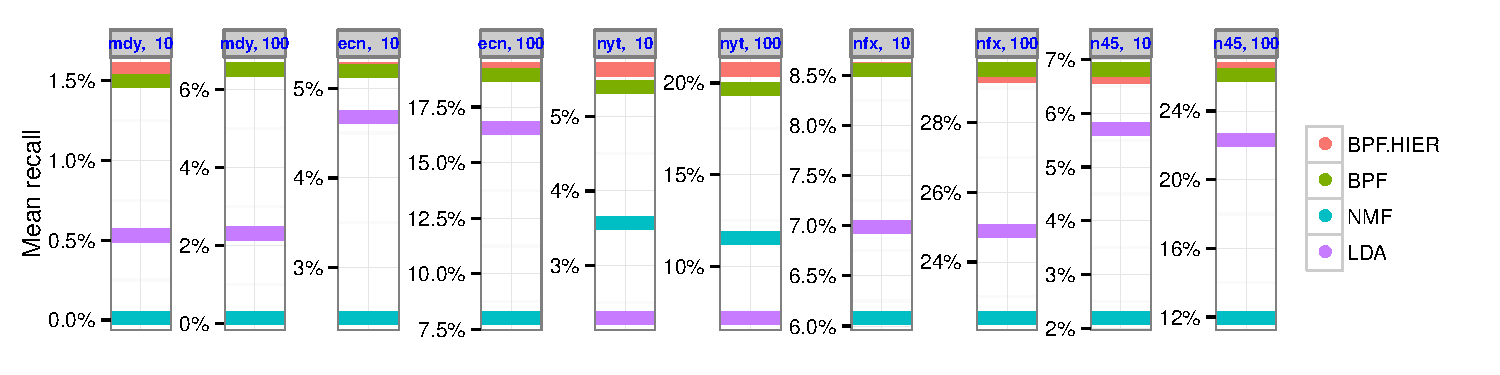
\includegraphics[width=\textwidth]{./figures/meanrecall2.pdf}\\               
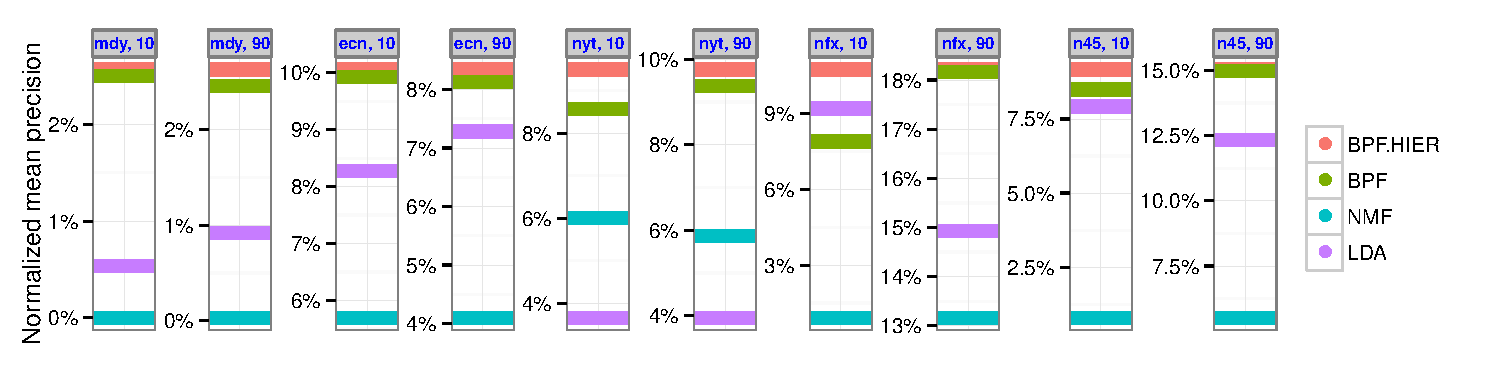
\includegraphics[width=\textwidth]{./figures/useractivity-meanprecision2.pdf}\\
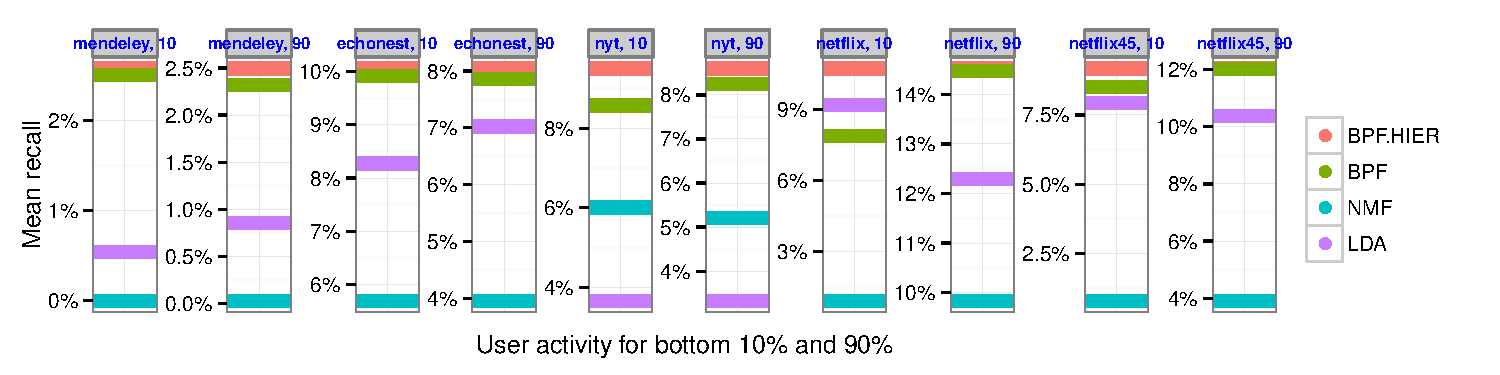
\includegraphics[width=\textwidth]{./figures/useractivity-meanrecall2.pdf}\\
\caption{Predictive performance on datasets. The top two plots show
  normalized mean precision and mean recall at 10 and 100
  recommendations. The bottom two plots show normalized mean precision
  and mean recall for the bottom 10\% and bottom 90\% of users by
  activity.}
\label{fig:precision_by_M}
\end{figure*}


\section{Empirical Study}
We studied the Bayesian Poisson Factorization (BPF) algorithm of
Figure~\ref{fig:batch} on a variety of large real data sets. We
demonstrate in this section that BPF definitively outperforms matrix
factorization (MF) in predictive performance on all data sets.
\begin{figure*}[th]
\centering
\subfigure[]{
  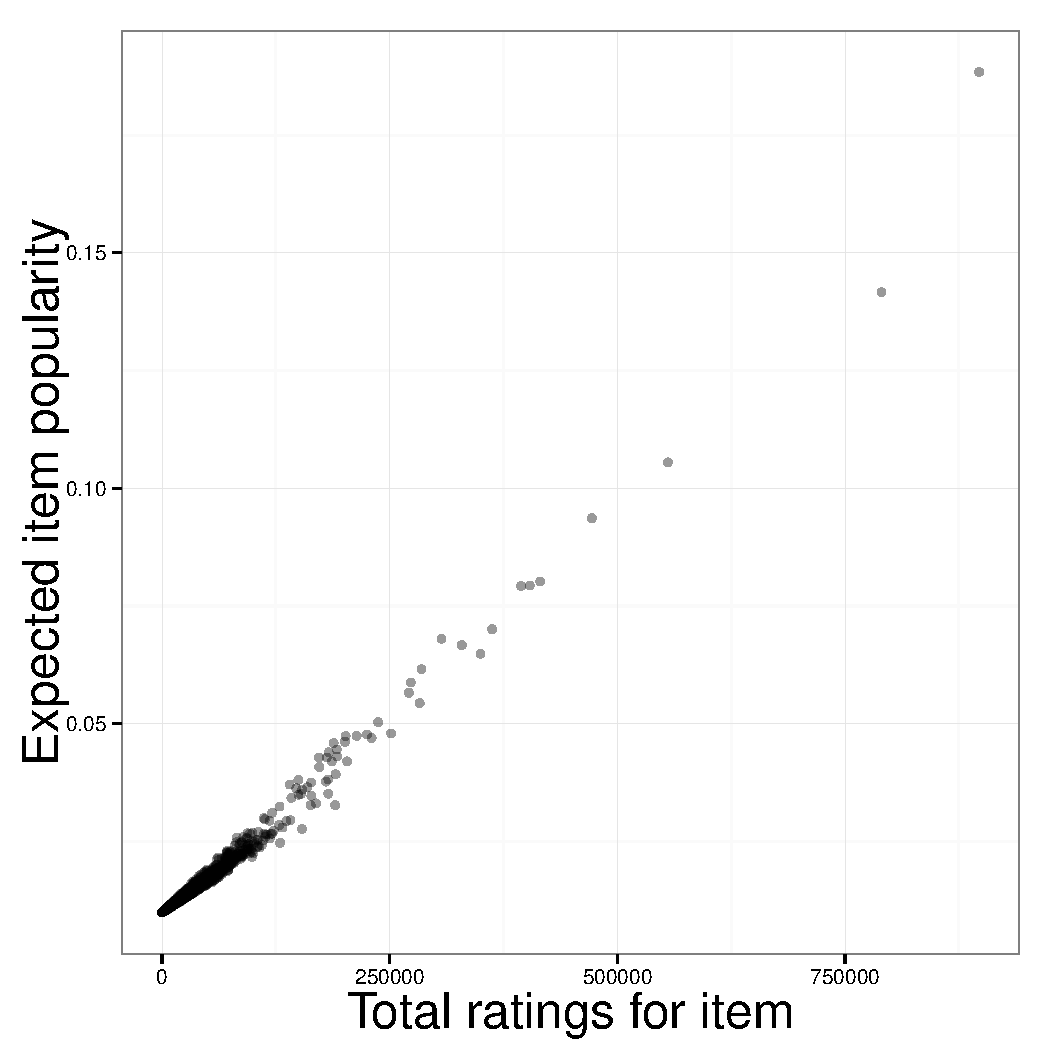
\includegraphics[width=0.45\textwidth]{./figures/nyt/itemsrate.pdf}
}
\subfigure[]{
  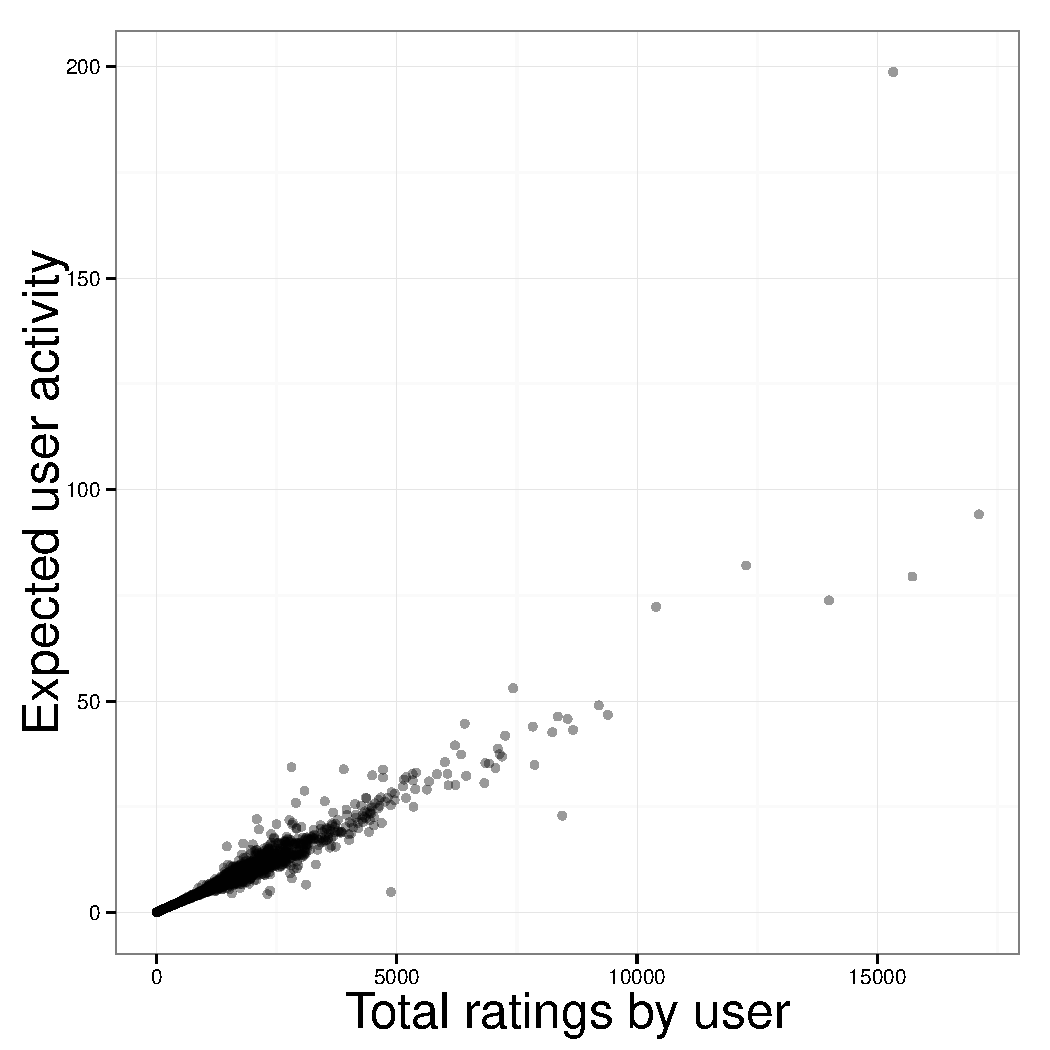
\includegraphics[width=0.45\textwidth]{./figures/nyt/userrate.pdf}
}
\caption{Popularity of articles on the NYT dataset.}
\label{fig:nyt-expl}
\end{figure*}


\begin{table*}
\centering
\caption{Most popular articles in the NYT dataset}
\begin{tabular}{|l|r|r|} \hline
Title & Expected popularity & Number of factors\\\hline
Blasts at Boston Marathon Kill 3 and Injure 100 & 0.043 & 1\\\hline
FBI Posts Images of Pair Suspected in Boston Attack & 0.042 & 1\\\hline
Bombing Inquiry Turns to Motive and Russia Trip & 0.037 & 1\\\hline
War Zone at Mile 26: 'So Many People Without Legs' & 0.025 & 1\\\hline
Suspects Seemed Set for Attacks Beyond Boston & 0.031 & 1\\\hline
In Signal Image From Boston Bombing a Father Sees His Son & 0.029 & 1\\\hline
Skeleton in British Parking Lot Hailed as Richard III & 0.027 & 4\\\hline
Surviving Suspect is Charged by US in Boston Attack & 0.027 & 1\\\hline
The Boy With A Thorn In His Joints & 0.026 & 3\\\hline
Drowned in a Stream of Prescriptions & 0.025 & 3\\\hline
\end{tabular} 
\end{table*}

{\bf Data Sets.} We study the Bayesian Poisson Factorization algorithm
in Figure~\ref{fig:batch} on several large data sets:
\begin{itemize}
\item The {\bf New York Times} data set with 1,615,675 users, 103390
  articles movies and 80,071,435 ratings.
\item The {\bf Netflix} data set~\cite{Koren:2009} with 480,000 users,
  17,770 movies and 100 million ratings is similar to MovieLens but
  significantly larger. Unlike the MovieLens data, the Netflix data
  set is highly skewed and is more realistic: Some users rate more
  than 10,000 movies, while others rate less than
  5~\cite{Salakhutdinov:2008a}.
\item The {\bf Mendeley} data set~\cite{Jack:2010} of scientific
  articles is a binary matrix of
  80,000 users and 260,000 articles, where an article is considered
  consumed by a user if it's in the user's library.
\item The {\bf Echo Nest} music data set~\cite{Bertin-Mahieux:2011} consists of 1
  million users, 385,000 distinct songs and 48 million (user, song,
  play count) triplets.
\end{itemize}

The scale and diversity of these data sets enables a robust evaluation
of our algorithm. Both the Mendeley and the Echo Nest data sets are
sparse in comparison to the movie data: only 0.001\% of the matrix of
ratings is non-zero in Mendeley, while 1\% of the ratings are non-zero
in Netflix and 4\% in MovieLens. Further, the Mendeley data set has
many more articles than users.


%% users watching movies on MovieLens~\cite{Koren:2009} and
%% Netflix~\cite{Herlocker:1999}, individuals listening to songs in the
%% Echo Nest data set~\cite{Bertin-Mahieux:2011}, and academics reading
%% scientific articles via Mendeley~\cite{Jack:2010}.


%% The MovieLens data set consists of 1 million ratings
%% from 6040 users on 4000 movies. Each movie is associated with a title
%% and a category. The Netflix data set is similar to---but significantly
%% larger than---the MovieLens data set, consisting of 100M ratings from
%% 480,000 users on 17770 movies.

{\bf Pre-processing and training.} We now describe how we the
pre-process the input data, train the model, and assess the predictive
accuracy on a held-out set.

Prior to training, we randomly select 20\% of ratings in each data set
to be used as a held-out test set comprised of items that the user
has consumed. During training, these test set observations are treated
as zeros. Additionally, we set aside 1\% of the training ratings as a
validation set and use it to determine the convergence of our
algorithm.

During training, the input to our algorithm is the count data, for
example, the movie ratings or the play count of a song. Notice that
for the Mendeley data set, the input is binary. During training, we
fix the shape and rate hyperparameters. This gives good performance on
our validation set. We find that the algorithm is insensitive to small
changes in the hyper-parameters.

%% corresponding to ratings or the play count of a song. Optionally, the
%% algorithm can transform the input count data to binary before training
%% the model.  For example, the observation $y_{ui}$ is set to one only
%% if the $u$-th user explicitly rated the $i$-th movie. (We denote the
%% algorithm that fits the transformed data, BPF-binary or BPF-BIN.)

We terminate the training process when the BPF algorithm
converges. The convergence is measured by computing the prediction
accuracy on our validation set. We approximate the probability that a
user consumed an item using the variational approximations to
posterior expectations of $\theta_u$ and $\beta_i$, and compute the
average predictive log likelihood of the validation ratings. The BPF
algorithm stops when the change in log likelihood is less than
0.0001\%.

{\bf Exploratory analysis.} The fitted model can be explored to
discover latent structure among items and users and to confirm that
the model is capturing the components in the data in a reasonable
way. For example, in \myfig{components} we illustrate the components
discovered by our algorithm on the MovieLens and the Netflix movie
ratings and the Mendeley data of users and scientific articles. For
each data set, the illustration shows the top 10 items---items sorted
in decreasing order of their expected weight $\beta_i$---from three of
the 100 components discovered by our algorithm. These components
naturally organize the movies and articles, and enable recommendation
of new items to the user.

In \myfig{movielens-illustration} we show a subset of the highly rated
movies of a user from the MovieLens data
set~\cite{Herlocker:1999}. The top 15 movies recommended to this user
using the trained BPF model, are also shown. The user's ratings are
for primarily drama movies. We movies BPF recommends closely resemble
the types of drama movies she is interested in, for example,
``Children's drama'' or ``War drama''. The expected user's $K$-vector
of weights $\theta_u$, inferred by our algorithm, is shown in
\myfig{movielens-illustration}. In our analysis, $K$ was set to
100. The $\theta_u$ are not sparse because the user's views span a
range of movies in the small data set.

{\bf Testing.} During testing, we generate the top $M$ recommendations
for each user as those items with the highest predictive score in
\myeq{score}. The ranked list of items predicted for each user
includes items in the test set, as well as items in the training set
that were zeros. We compute precision-at-$M$, which measures the
fraction of the top $M$ recommendations present in the test set,
varying $M$ from 10 to 100 items. Likewise, we compute recall-at-$M$,
which captures the fraction of items in the test set present in the
top $M$ recommendations.

%% In contrast, the Echo Nest and Mendeley data sets contain implicit
%% feedback on which songs and scientific papers users have consumed.

%% !!! prem: assume BPF-binary for now. will try to move to BPF-bias
%% where the non-binary observations are fit

{\bf Baselines.} We compare our performance against traditional matrix
factorization (MF). Ratings are modeled as
\begin{equation*}
  y_{ui} = c + a_u + b_i + \theta_u^\top \beta_i,
\end{equation*}
where $c$ denotes a global intercept term, $a_u$ captures the relative
activity of the $u$-th user, and $b_i$ accounts for the popularity of
the $i$-th item. The final term quantifies interactions between a user
and item via their K-dimensional latent factors, with $\theta_u$ specifying
the user's interests and $\beta_i$ describing the item's attributes. The
model is fit by stochastic gradient descent using the open source
Vowpal Wabbit package~\cite{Weinberger:2009} to minimize squared error
between predicted and actual ratings.

We note that while BPF takes only the non-zero observed ratings as
input, traditional matrix factorization requires that we provide
explicit zeros in the ratings matrix as negative examples. In
practice, this amounts to either treating all missing ratings as zeros
and down-weighting to balance the relative importance of observed and
missing ratings~\cite{Hu:2008p9402}, or generating negatives by
randomly sampling from missing ratings in the training
set~\cite{Dror:2012a}.  We take the latter approach for computational
convenience, employing two popular sampling schemes. In the first,
denoted MF-UNI, we sample a fixed number of negative examples
uniformly at random for each user such that there are approximately
the same number of positive and negative examples. In the second,
termed MF-POP, we sample users by activity---the number of items rated
in the training set---and items by popularity---the number of training
ratings an item received. 

For MF, we cross-validate over the gradient update step size, the
strength of an $L_2$-regularization term across all weights, and the
number of passes over the training data. This results in a reasonably
expensive grid search, from which we select
the model that performs best on the validation set for each data set.

%% \begin{figure*}[t]
%% \centering
%% \includegraphics[width=\textwidth]{./figures/precision_by_user_activity_and_method.pdf}\\
%% \label{fig:precision_by_user_activity}
%% \caption{Precision at 100 recommendations by user activity across data sets and methods.}
%% \end{figure*}

%% \begin{figure*}
%% \centering
%% 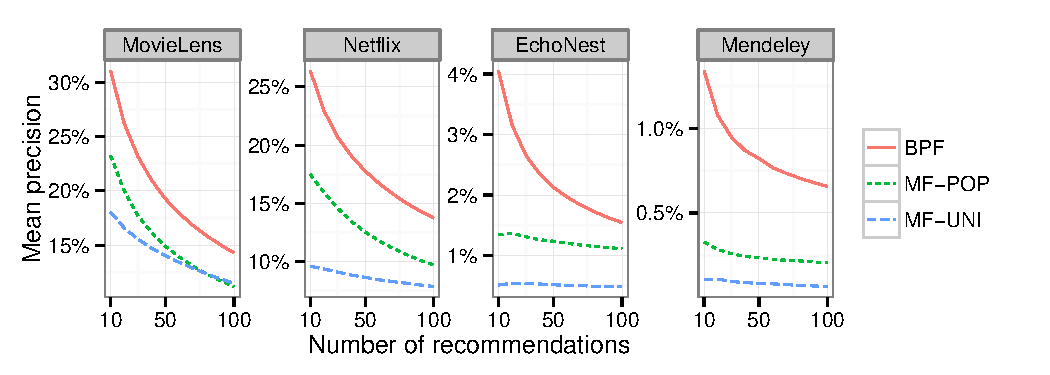
\includegraphics[width=\textwidth]{../output/figures/echonest_and_mendeley/mean_precision_by_method.pdf}\\
%% \includegraphics[width=\textwidth]{../output/figures/echonest_and_mendeley/precision_by_user_activity_and_method.pdf}\\
%% \includegraphics[width=\textwidth]{../output/figures/echonest_and_mendeley/mean_coverage_by_method.pdf}\\
%% \end{figure*}

%% {\bf Results and analysis.} \myfig{precision_by_M} shows the mean
%% precision of the BPF and the MF algorithm as we vary $M$, the number
%% of recommendations. As shown in \myfig{precision_by_M}, BPF
%% outperforms MF on all data sets by a sizeable margin---as much as 8
%% percentage points. Likewise, BPF shows similar gains in recall over
%% traditional MF approaches, indicated in \myfig{recall_by_M}. A
%% relatively high fraction of items recommended by BPF are found to be
%% relevant, and many relevant items are recommended.

%% We also study precision as a function of user activity to investigate
%% for which kinds of users the algorithm performs
%% well. \myfig{precision_by_user_activity} highlights the results in
%% further detail, showing the precision at 100 recommendations for users
%% of varying activity. BPF provides increasingly better performance for
%% more active users.  On the Mendeley data set, BPF performs better for
%% users with less than 1000 articles (BPF does better over all.)  On all
%% other data sets, BPF performs better than MF with all types of users.

%% In all results, MF-POP outperforms MF-UNI, which is indicative of
%% problems with the squared loss objective approximated by MF-UNI.

%% As expected, we see that BPF provides
%% increasingly better recommendations for more active users, and that
%% BPF outperforms MF on the Netflix, MovieLens, and Echo Nest data sets
%% by this measure as well as mean precision across all users.

%% On the Mendeley data set, BPF performs better for users with less than
%% 1000 articles in their library, but MF has better precision than BPF for
%% the small set of users with more than 1000 papers in their library. 

%% !!! prem: need to confirm by looking at actual values; investigate
%\newpage

\begin{figure*}
\centering
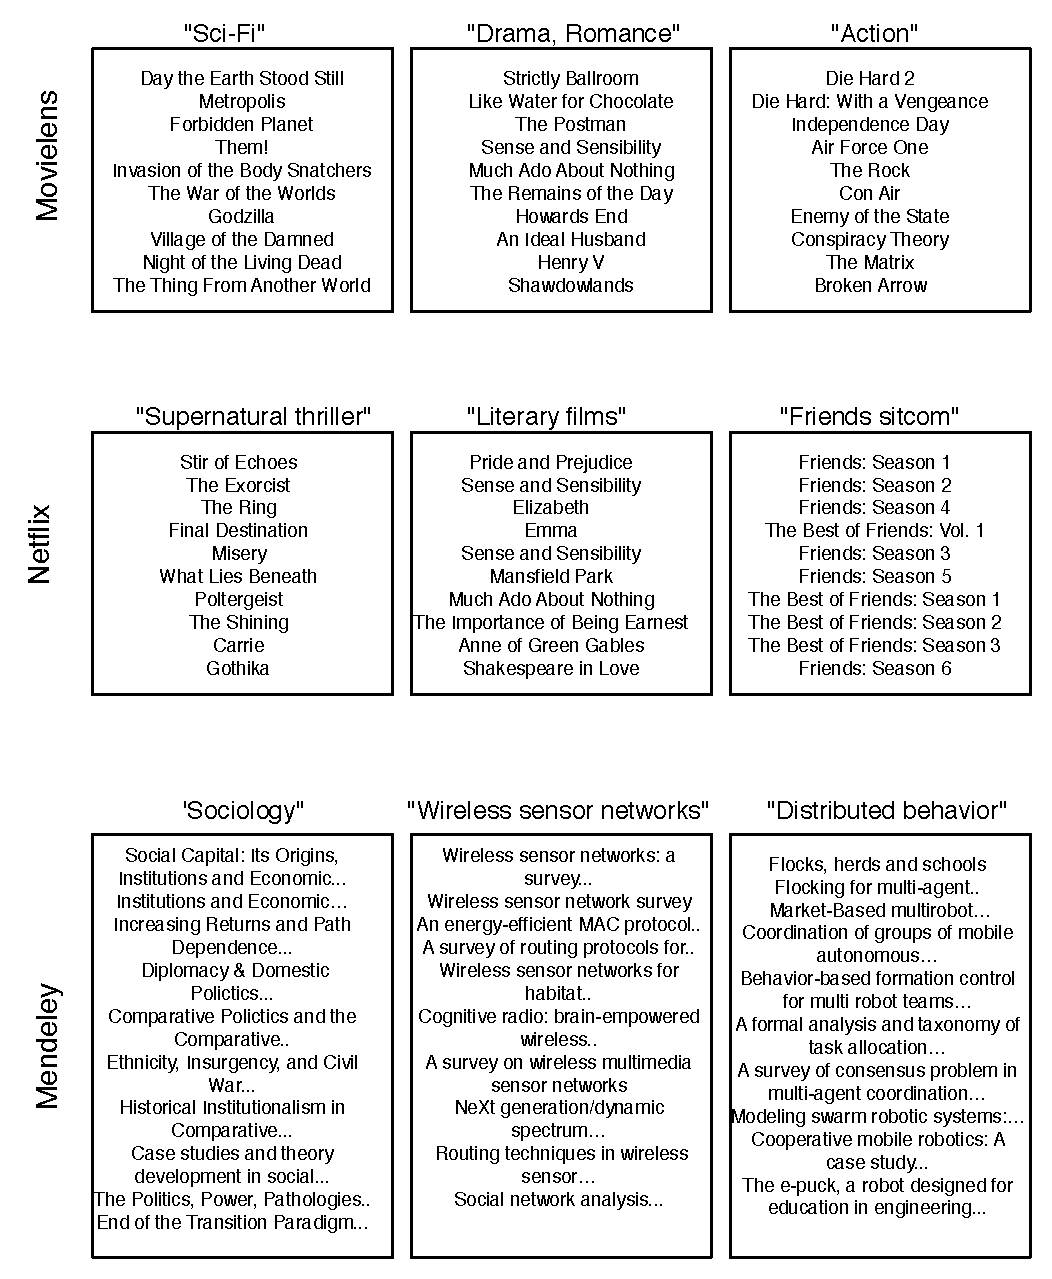
\includegraphics[width=\textwidth]{./figures/components.pdf}
\caption{The top 10 items by the expected weight $\beta_i$ from three
  of the 100 components discovered by our algorithm.}
\label{fig:components}
\end{figure*}
